%%%%%%%%%%%%%%%%%%%%%%%%%%%%%%%%%%%%%%%%%
% University/School Laboratory Report
% LaTeX Template
% Version 3.1 (25/3/14)
%
% This template has been downloaded from:
% http://www.LaTeXTemplates.com
%
% Original author:
% Linux and Unix Users Group at Virginia Tech Wiki 
% (https://vtluug.org/wiki/Example_LaTeX_chem_lab_report)
%
% License:
% CC BY-NC-SA 3.0 (http://creativecommons.org/licenses/by-nc-sa/3.0/)
%
%%%%%%%%%%%%%%%%%%%%%%%%%%%%%%%%%%%%%%%%%

%----------------------------------------------------------------------------------------
%	PACKAGES AND DOCUMENT CONFIGURATIONS
%----------------------------------------------------------------------------------------

\documentclass{article}
\usepackage[utf8]{inputenc}
\usepackage{appendix}
\usepackage[T1]{fontenc}
\usepackage{siunitx} % Provides the \SI{}{} and \si{} command for typesetting SI units
\usepackage{graphicx} % Required for the inclusion of images
\usepackage{natbib} % Required to change bibliography style to APA
\usepackage{amsmath} % Required for some math elements 
\usepackage{caption}
\usepackage{tikz}

\usetikzlibrary{arrows,automata, positioning}

\usepackage{import}

\setlength\parindent{0pt} % Removes all indentation from paragraphs

%\renewcommand{\labelenumi}{\alph{enumi}.} % Make numbering in the enumerate environment by letter rather than number (e.g. section 6)

%\usepackage{times} % Uncomment to use the Times New Roman font

%----------------------------------------------------------------------------------------
%	DOCUMENT INFORMATION
%----------------------------------------------------------------------------------------

\title{Prova Finale di Reti Logiche} % Title
\author{Truong Kien Tuong} % Author name
\date{May 1st, 2020}

\begin{document}
\maketitle % Insert the title, author and date
\begin{center}
\begin{tabular}{l r}
Matricola: & 887907\\ % Partner names
Codice Persona: & 10582491\\
Docente: & Gianluca Palermo % Instructor/supervisor
\end{tabular}
\end{center}

% If you wish to include an abstract, uncomment the lines below
% \begin{abstract}
% Abstract text
% \end{abstract}

%----------------------------------------------------------------------------------------
%	SECTION 1
%----------------------------------------------------------------------------------------

\section{Requisiti del Progetto}

Il progetto richiesto consiste nell'implementazione in VHDL del metodo di codifica basato sulle \textbf{"Working Zones"} (Abbr. WZ).\\
Dato un indirizzo di memoria su 7 bit (8 di cui il primo è settato a zero)
e l'indirizzo di 8 blocchi di memoria da 4 celle, detti "Working Zones",
viene richiesto al componente di:
\begin{enumerate}
\item Accedere ad una memoria RAM per recuperare i dati sopra descritti
\item Verificare se l'indirizzo di memoria appartiene ad una delle working zones
	\begin{enumerate}
	\item Se sì, codificare l'indirizzo settando il primo bit a 1, i successivi 3 bit al numero della WZ codificato in binario
	e gli ultimi 4 bit alla codifica one-hot della posizione dell'indirizzo nella WZ
	\item Altrimenti, restituire l'indirizzo come è stato fornito, con il primo bit a 0.
	\end{enumerate}
\item Scrivere il risultato nella memoria RAM
\end{enumerate}

Inoltre, l'implementazione deve essere in grado di gestire un segnale di Reset.
Per l'implementazione si è scelto di supporre il Reset asincrono rispetto al segnale di clock.

L'implementazione deve essere poi sintetizzata con target FPGA xc7a200tfbg484-1.

\subsection{Esempio}
Si riporta in seguito un esempio di codifica con il metodo delle Working Zones. Nella figura è riportata una memoria con indirizzamento a 8 bit (Gli indirizzi sono rappresentati nella memoria tra parentesi quadre) con una working zone (WZ5) con indirizzo di partenza $00101000$.
\newpage
Gli indirizzi contenuti nella working zone riportano a lato il relativo offset rispetto all'indirizzo di partenza tra parentesi tonde.

Nella figura è illustrato un esempio in cui l'indirizzo è effettivamente contenuto in una WZ, in modo da esplicitare come deve essere effettuata la codifica.

%\vspace*{\fill}
\vspace*{1cm}
\noindent
\makebox[\textwidth]{
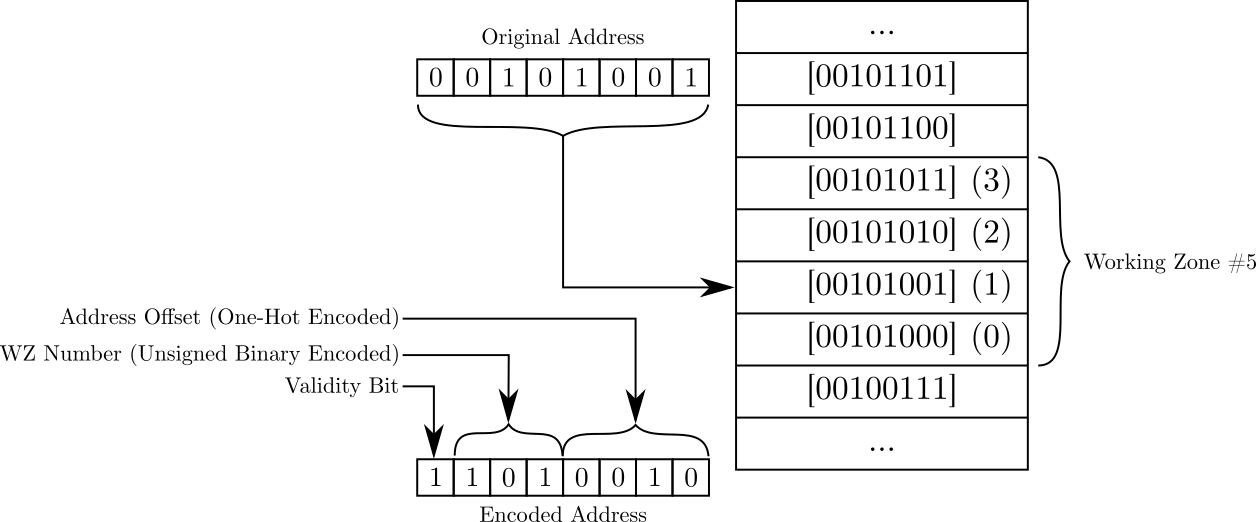
\includegraphics[scale=0.5]{./pictures/specification.png}}%
\captionof{figure}{Esempio di codifica di indirizzo contenuto in una Working Zone}
\vspace*{0.5cm}

\subsection{Ipotesi Progettuali}
\label{ipotesi}
Si sono supposti veri i seguenti fatti:
\begin{enumerate}
\item Le WZ non possono mai sovrapporsi (i.e. Non possono esistere due WZ tali che l'indirizzo di una sia all'interno dell'altra WZ). Si è scelto di
supporre ciò per evitare ambiguità nella codifica dell'indirizzo.
\item Non possono esistere WZ malformate (i.e Non può esistere una WZ che, nel range di indirizzi da 0 a 127, abbia meno di 4 celle).
\end{enumerate}
 
%----------------------------------------------------------------------------------------
%	SECTION 2
%----------------------------------------------------------------------------------------

\section{Implementazione}

L'architettura è stata progettata in maniera modulare, in modo da specializzare i singoli componenti creati e separare le funzionalità
di calcolo della codifica dell'indirizzo dalla gestione della macchina a stati finiti.

\subsection{Descrizione ad Alto Livello}
\label{alto_livello}

Da un'ottica di alto livello, l'implementazione esegue i seguenti passi:

\begin{enumerate}
\item Carica l'indirizzo da codificare dalla RAM in una memoria interna
\item Se le Working Zones non sono ancora state tutte caricate:
	\begin{enumerate}	
	\item Carica l'indirizzo della WZ dalla RAM
	\item Verifica se il nuovo indirizzo della WZ contiene l'indirizzo da codificare
	\item Se sì, setta il risultato all'indirizzo codificato e salta a 4
	\item Altrimenti torna a 2
	\end{enumerate}
\item Controlla se dal caricamento dell'ultima WZ è stato ottenuto un risultato
	\begin{enumerate}
	\item Se sì, setta il risultato a tale indirizzo codificato
	\item Altrimenti, setta il risultato all'indirizzo originale
	\end{enumerate}
\item Scrive il risultato nella RAM
\item Se è richiesto un reset, torna a 1, altrimenti mantiene tutte le WZ e richiede solamente l'indirizzo
\item Carica il nuovo indirizzo da codificare 
\item Carica il risultato nella RAM e torna al punto 5
\end{enumerate}

Per gestire questo algoritmo si è scelta un'implementazione costituita da 3 tipi di entità: una macchina a stati finiti, che rappresenta il top-level component
e che gestisce il salvataggio nei registri degli stati e l'esecuzione delle transizioni, un Address Offset Units Controller e 8 Address Offset Units.
Segue una descrizione dettagliata di tutte le entità riportate.

\subsection{Address Offset Unit}
\label{AOU}

Il componente denominato \textbf{Address Offset Unit} (AOU) è un circuito combinatorio che, ricevuto un indirizzo di WZ \texttt{i\_wzaddress} e l'indirizzo da codificare \texttt{i\_address} verifica se l'indirizzo da codificare sia contenuto nella WZ.\\
Nel caso in cui la risposta sia positiva, calcola anche l'indirizzo codificato\\
\texttt{o\_address}, altrimenti restituisce un indirizzo interamente settato a 0.\\

La struttura modulare di tali componenti garantisce una facile estensione\\
dell'implementazione, se ciò risultasse necessario.
Inoltre, poichè verranno istanziate 8 AOU uguali (eccetto per il numero di WZ), si ottiene un'architettura simile ad un array sistolico, in grado di effettuare la computazione su tutte le 8 WZ
contemporaneamente e sfruttando così il parallelismo hardware fornito dall'FPGA.\\

Infine, un'architettura di questo genere ben si adatta al problema, che richiede una computazione di tipo SIMD (Single Instruction Multiple Data), con un layer di reduce dato dal Controller.\\

L'architettura dell'AOU è stata implementata con una specifica behavioural

\subsection{Address Offset Units Controller}
\label{Controller}

L'\textbf{Address Offset Units Controller} (AOU Controller) è un circuito combinatorio che interfaccia la macchina a stati finiti con le 8 AOU, istanziando quest'ultime
mediante un'istruzione generate in VHDL. A ciascuna AOU è assegnato un numero di WZ mediante generic mapping.
Il process del Controller verifica per ciascun AOU se:

\begin{enumerate}
\item È stato ottenuto un risultato valido dall'AOU (Ovvero l'indirizzo da codificare appartiene alla WZ assegnata)
\item La WZ assegnata è valida (Ovvero è aggiornata allo stato attuale dei dati contenuti nella RAM)
\end{enumerate}

La seconda condizione è necessaria per consentire l'esistenza di una WZ che inizia all'indirizzo 0. Se non si tenesse conto della validità della WZ, subito dopo il reset
si avrebbe che tutte le AOU possiedono un risultato valido (Dato dall'indirizzo da codificare \texttt{0x00} che è banalmente contenuto in una WZ che inizia in \texttt{0x00}).

Non appena il Controller ha trovato un risultato valido, questo viene asserito come output. Se non viene trovato alcun risultato valido dalle AOU, viene asserito
l'indirizzo in ingresso come output.

L'architettura dell'AOU Controller è stata implementata con una specifica in parte strutturale, data dai collegamenti con le AOU, e in parte comportamentale,
nella gestione dei risultati delle AOU.

\subsection{Macchina a Stati Finiti}
\label{FSM}

La \textbf{Macchina a Stati Finiti} (FSM) è il circuito che si occupa di gestire lo stato della computazione e che si interfaccia con la RAM per il trasferimento dei dati.
La FSM è stata realizzata con specifica behavioural mediante due processi: \texttt{STATE\_OUTPUT} e \texttt{DELTA\_LAMBDA}.

Il processo \texttt{STATE\_OUTPUT} è il processo sequenziale che ha il compito di asserire le uscite e di cambiare lo stato interno sul fronte di salita del clock.
Il processo \texttt{DELTA\_LAMBDA} è invece il processo combinatorio che calcola le uscite e lo stato validi per il prossimo fronte di salita.

Segue una descrizione degli stati formali della FSM:

\begin{itemize}
\item \texttt{IDLING}: Stato di idle in cui si posiziona la FSM al reset della computazione. La macchina aspetta che venga asserito il segnale \texttt{i\_start}.
\item \texttt{SET\_READ\_ADDR}: Stato in cui vengono preparate le uscite per leggere l'indirizzo da codificare dalla RAM
\item \texttt{WAIT\_READ\_ADDR}: Stato in cui si aspetta un ciclo di clock per consentire alla RAM di asserire le sue uscite
\item \texttt{FETCH\_DATA\_ADDR}: Stato in cui si legge il dato dalla RAM e viene salvato l'indirizzo da codificare
\item \texttt{SET\_READ\_WZ}: Stato in cui vengono preparate le uscite per leggere l'indirizzo della i-esima WZ
\item \texttt{WAIT\_READ\_WZ}: Stato in cui si aspetta un ciclo di clock per consentire alla RAM di asserire le sue uscite 
\item \texttt{FETCH\_DATA\_WZ}: Stato in cui si legge il dato dalla RAM e viene salvato l'indirizzo della i-esima WZ
\item \texttt{WAIT\_RESULT}: Stato in cui, dopo il caricamento di tutte le WZ, si aspetta un ciclo di clock per consentire la propagazione dei dati nell'AOU Controller
\item \texttt{SET\_WRITE}: Stato in cui vengono preparate le uscite per scrivere il risultato nella RAM e si asserisce \texttt{o\_done} a 1
\item \texttt{END\_WRITE}: Stato in cui si aspetta che \texttt{i\_start} venga portato giù, settando \texttt{o\_done} a 0 e riportandosi allo stato di \texttt{IDLING}.
\end{itemize}

Più precisamente l'insieme degli stati della FSM dovrebbe comprendere almeno anche il counter \texttt{CURR\_WZ}, che assume come valore il numero della WZ che deve essere caricata.
Così facendo gli stati \texttt{SET\_READ\_WZ}, \texttt{WAIT\_READ\_WZ} e \texttt{FETCH\_DATA\_WZ} sarebbero, dunque, da replicare per tutte le 8 WZ.\\

Nella figura a seguito è riportato il disegno dell'automa. Sono state usate le seguenti abbreviazioni degli stati per chiarezza:\\

\begin{center}
\begin{tabular}{ll}
\texttt{IDLING}: & \texttt{IDLE}\\
\texttt{SET\_READ\_ADDR}: & \texttt{SR\_ADDR} \\
\texttt{WAIT\_READ\_ADDR}: & \texttt{WR\_ADDR} \\
\texttt{FETCH\_DATA\_ADDR}: & \texttt{FD\_ADDR} \\
\texttt{SET\_READ\_WZ} (With \texttt{WZ\_COUNT=i}): & \texttt{SR\_WZ\_i} \\
\texttt{WAIT\_READ\_WZ} (With \texttt{WZ\_COUNT=i}): & \texttt{WR\_WZ\_i} \\
\texttt{FETCH\_DATA\_WZ} (With \texttt{WZ\_COUNT=i}): & \texttt{FD\_WZ\_i} \\
\texttt{WAIT\_RESULT}: & \texttt{WAIT\_RES} \\
\texttt{SET\_WRITE}: & \texttt{SET\_WR} \\
\texttt{END\_WRITE}: & \texttt{END\_WR} \\
\end{tabular}
\end{center}


\begin{center}
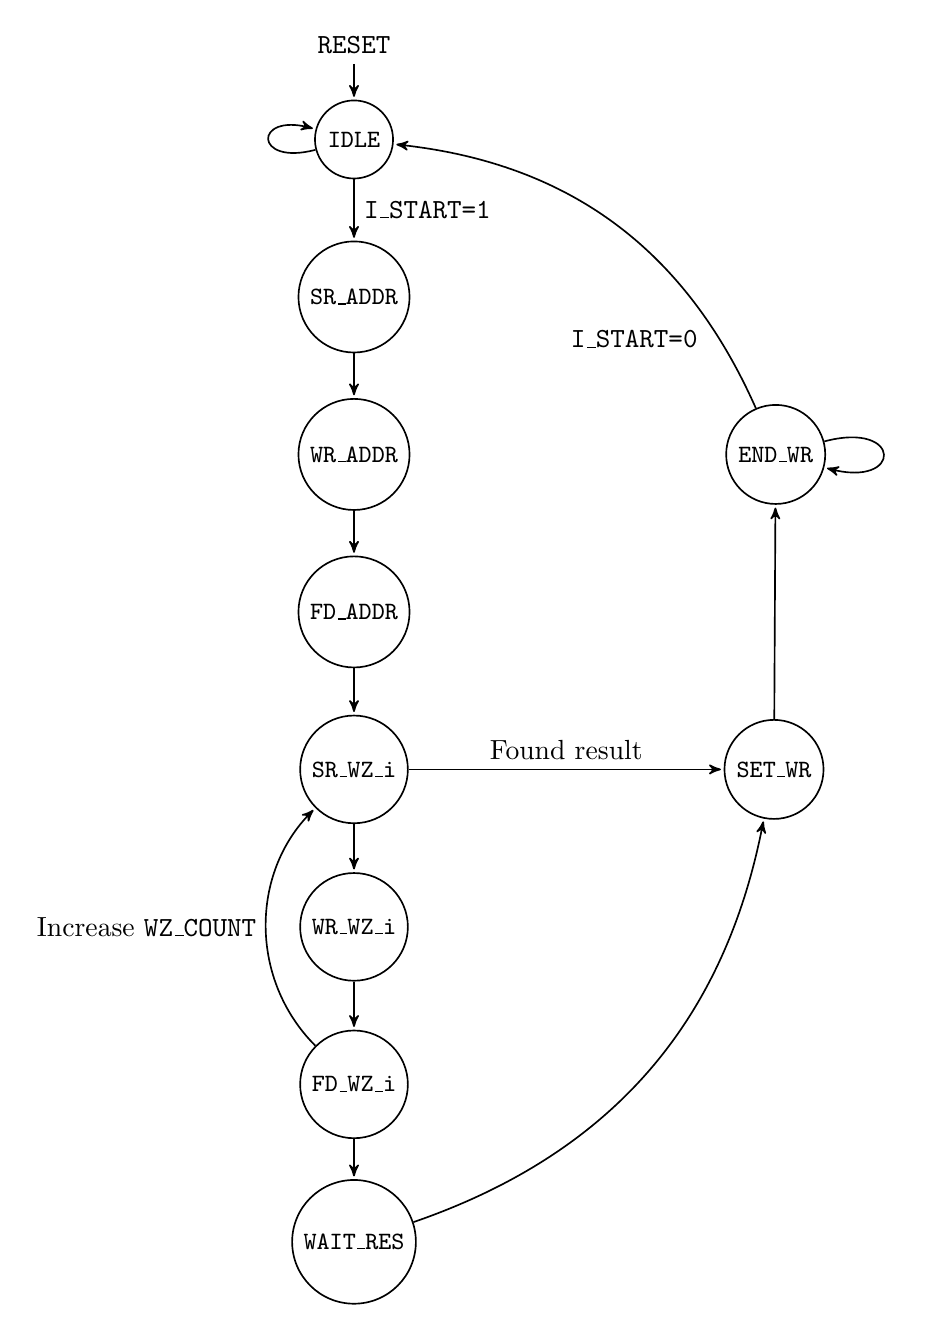
\begin{tikzpicture}[->,>=stealth',shorten >=1pt,auto,node distance=2cm,
                    semithick, initial where=above, initial text={\texttt{RESET}}]

  \tikzstyle{every state} = [font=\small]
  \node[initial,state] (A)                    {\texttt{IDLE}};
  \node[state]         (B) [below of=A] 	  {\texttt{SR\_ADDR}};
  \node[state]         (C) [below of=B] 	  {\texttt{WR\_ADDR}};
  \node[state]         (D) [below of=C] 	  {\texttt{FD\_ADDR}};
  \node[state]         (E) [below of=D]       {\texttt{SR\_WZ\_i}};
  \node[state]         (F) [below of=E]       {\texttt{WR\_WZ\_i}};
  \node[state]         (G) [below of=F]       {\texttt{FD\_WZ\_i}};
  \node[state]         (H) [below of=G]       {\texttt{WAIT\_RES}};
  \node[state]         (I) [right=4cm of E]       {\texttt{SET\_WR}};
  \node[state]         (J) [right=4cm of C]       {\texttt{END\_WR}};

  \path (A) edge              node [pos=0.5]{\texttt{I\_START=1}} (B)
 	    (A) edge  [loop left] node {} (A)
        (B) edge              node {} (C)
        (C) edge              node {} (D)
        (D) edge 			  node {} (E)
        (E) edge 			  node {} (F)
        (F) edge 			  node {} (G)
        (G) edge 			  node {} (H)
        (H) edge	[bend right]		  node {} (I)
        (I) edge			  node {} (J)
        (E) edge			  node {Found result} (I)
        (J) edge	[bend right]		  node [pos=0.2] {\texttt{I\_START=0}} (A)
        (J) edge	[loop right]		  node {} (J)
        (G) edge	[bend left=45]		  node {Increase \texttt{WZ\_COUNT}} (E);
        
\end{tikzpicture}
\end{center}
\captionof{figure}{Diagramma degli stati della Macchina a Stati Finiti}

\newpage

Si noti come il fatto di poter dare il risultato anche durante la fase di setup nasconde parte del tempo impiegato per caricare le WZ, riuscendo a fornire il risultato non appena si hanno i dati per poterlo calcolare.

\subsection{Schema dell'Implementazione}
\label{schema}

\vspace*{1cm}

% Your image goes here
\noindent
\makebox[\textwidth]{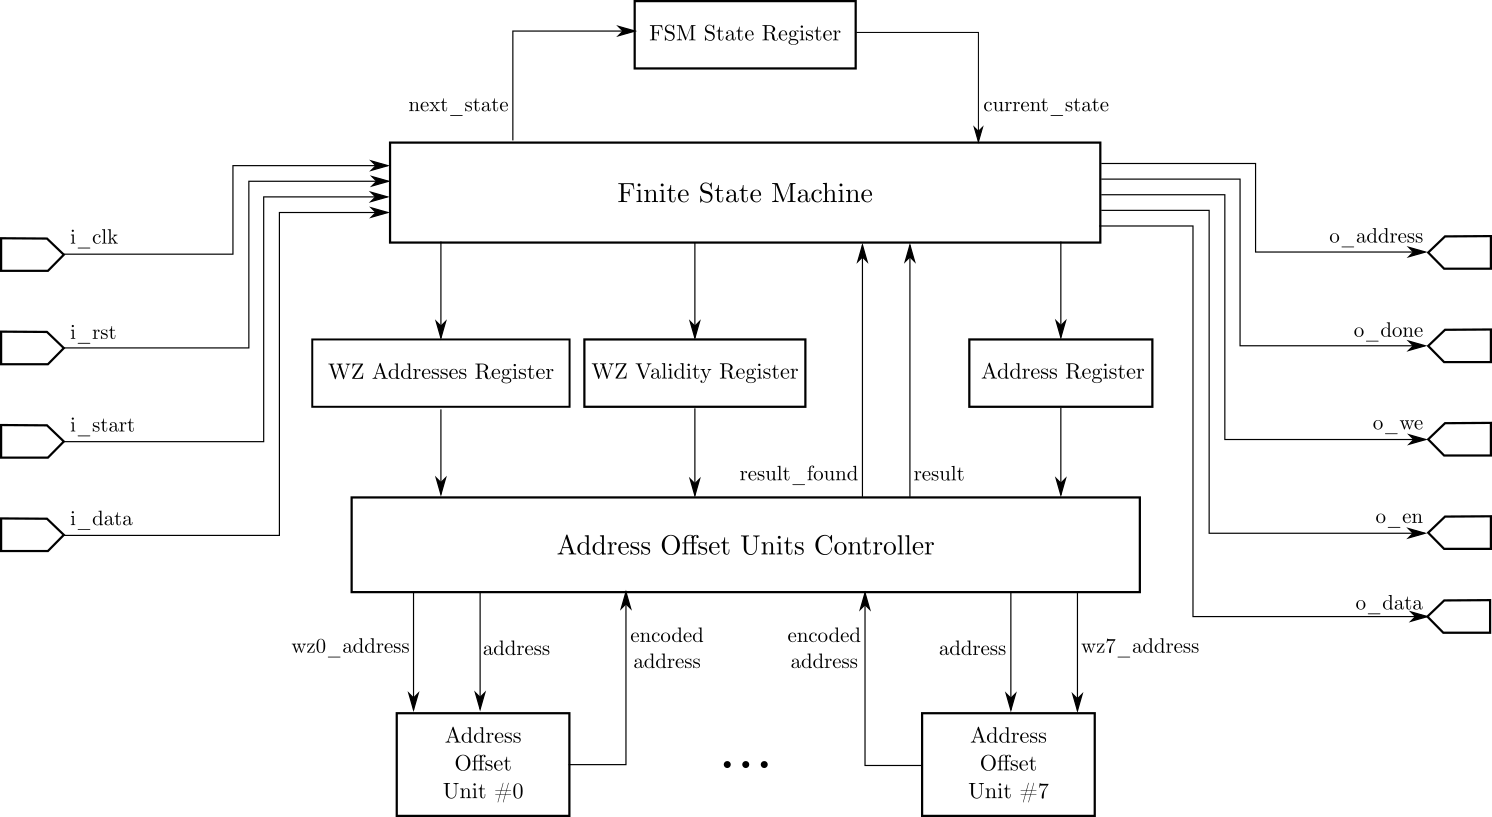
\includegraphics[scale=0.5]{./pictures/schematic.png}}%
\captionof{figure}{Schema ad alto livello dell'implementazione}

\vspace*{1cm}



%----------------------------------------------------------------------------------------
%	SECTION 3
%----------------------------------------------------------------------------------------

\section{Test Benches}
\label{test}

I test effettuati hanno cercato di effettuare transizioni critiche oppure di verificare possibili configurazioni di memoria estreme. In particolare sono stati creati dei testbench
comprendenti le seguenti situazioni:

\begin{itemize}
\item Segnale di \texttt{RESET} dopo che la macchina ha asserito il segnale di \texttt{o\_done} ma prima del segnale di \texttt{i\_start}
\item Ultima WZ all'indirizzo \texttt{0x00} e indirizzo da codificare \texttt{0x00}, test particolarmente importante per le ragioni fornite prima sul funzionamento dell'AOU Controller.
\item Ultima WZ all'indirizzo \texttt{0x7C} (Ovvero \texttt{0b01111100}, l'ultimo indirizzo possibile per una WZ) e indirizzo da codificare \texttt{0x7F} (Ovvero \texttt{0b01111111})
\item Altri test bench vari generati casualmente, mantenendo la validità della specifica
\item 10000 indirizzi da codificare con sempre le stesse WZ e senza mai effettuare reset (\texttt{KEEP WZs})
\item Gli stessi 10000 indirizzi da codificare e con sempre le stesse WZ ma con un reset dopo ogni indirizzo (\texttt{RESET WZs})
\end{itemize}

Questi test hanno evidenziato alcune criticità nel codice iniziale e hanno guidato lo sviluppo della soluzione fino alla sua versione finale.\\

Per tutti i test riportati e i test successivi è stata effettuata la simulazione behavioural e successivamente la simulazione functional e timing post-synthesis, tutte con successo.\\

I risultati rilevanti sono riportati nella sezione \ref{risultati}.

\section{Risultati Sperimentali}
\label{risultati}

\subsection{Report di Sintesi}

Dal punto di vista dell'area la sintesi riporta il seguente utilizzo dei componenti:
\begin{itemize}
\item LUT: 197 (0.15\% del totale)
\item FF: 108 (0.04\% del totale)
\end{itemize}
Si è fatta particolare cautela nella scrittura del codice per evitare utilizzo di Latch.

\subsection{Risultato dei Test Bench}

Lavorando sul testing si è anche provato a variare il periodo di clock, confermando che, non solo l'implementazione rispetta le specifiche, funzionando a \SI{100}{\ns},
ma mantiene il suo funzionamento anche a \SI{1}{\ns} nella simulazione Behavioural e \SI{7}{\ns} nella simulazione Functional Post-Synthesis.\\

Si riportano i risultati di tempo legati agli ultimi 2 test riportati nella sezione \ref{test}\\

\begin{tabular}{ll}
Simulazione KEEP WZs (Functional Post-Synthesis): & \SI{2020868600}{\ps}\\
Simulazione RESET WZs (Functional Post-Synthesis): & \SI{2754167600}{\ps}\\
\end{tabular}

\bigskip
Il risultato esprime una variazione del 36\% dal caso senza reset al caso con reset, evidenziando come l'architettura, per scelta progettuale,
è molto più efficiente quando non deve fare frequentemente la fase di setup, ossia la fase di caricamento delle WZ.

%----------------------------------------------------------------------------------------
%	SECTION 4
%----------------------------------------------------------------------------------------

\section{Conclusioni}

Si ritiene che l'architettura progettata rispetti anzitutto le specifiche, fatto che è stato verificato mediante estensivo testing sia casuale, che con test benches
manualmente scritti. Oltre a ciò l'architettura è stata pensata cercando di sfruttare al meglio il contesto in cui viene effettuata la computazione, ovvero quella
di parallelizzare il più possibile il lavoro effettuato dal componente.\\

Dal punto di vista del design, scegliere un'architettura modulare e facilmente espandibile è un vantaggio, anche nell'ottica di un'implementazione System on Chip,
in quanto consente di riutilizzare più volte lo stesso identico componente.

%----------------------------------------------------------------------------------------

\end{document}